\documentclass[tikz,border=5pt]{standalone}
\usetikzlibrary{calc}

\begin{document}
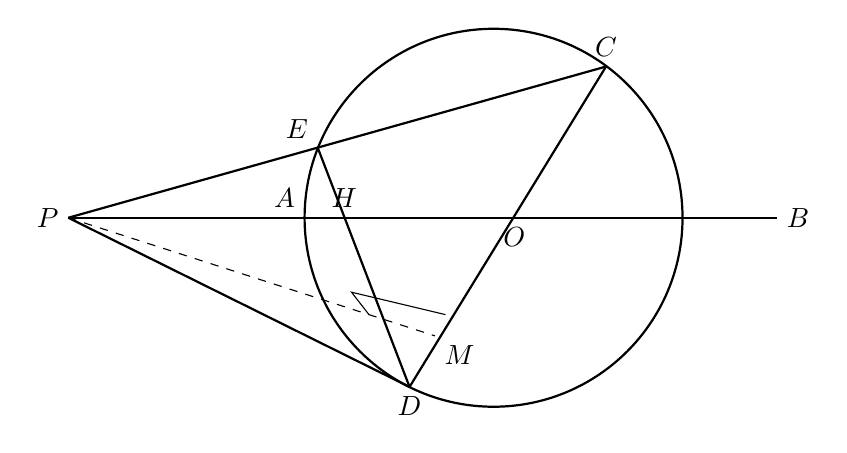
\begin{tikzpicture}[scale=1.2,>=stealth,
  dot/.style={circle,fill,inner sep=0pt,minimum size=2pt}]

  % main coordinates
  \coordinate (P) at (-4.5,0);
  \coordinate (O) at (0,0);
  \coordinate (A) at (-2,0);
  \coordinate (B) at (3,0);
  \coordinate (E) at (-1.86,0.74);
  \coordinate (C) at (1.19,1.60);
  \coordinate (D) at (-0.889,-1.79);

  % intersection of ED with PB (labeled H after edit)
  \coordinate (Mpt) at (-1.58,0);

  % foot point on OD for dashed line (labeled M after edit)
  \coordinate (Hpt) at (-0.62,-1.25);

  % circle
  \draw[thick] (O) circle (2);

  % secant line P-E-C
  \draw[thick] (P) -- (C);

  % line P-B through O
  \draw[thick] (P) -- (B);

  % tangent P-D
  \draw[thick] (P) -- (D);

  % chord E-D
  \draw[thick] (E) -- (D);

  % segment C-D through O
  \draw[thick] (C) -- (D);

  % dashed perpendicular P to OD
  \draw[dashed] (P) -- (Hpt);

  % right angle mark at Hpt (between dashed line and OD)
  \draw ($(Hpt)!0.18!(P)$) -- ($($(Hpt)!0.18!(P)$)!0.18!90:(O)$) -- ($(Hpt)!0.18!(O)$);

  % labels
  \node[left] at (P) {$P$};
  \node[above left] at (E) {$E$};
  \node[above] at (C) {$C$};
  \node[above left] at (A) {$A$};
  \node[right] at (B) {$B$};
  \node[below] at (D) {$D$};
  \node[below right] at (O) {$O$};

  % swapped labels: point at ED∩PB now labeled H, foot now labeled M
  \node[above] at (Mpt) {$H$};
  \node[below right] at (Hpt) {$M$};

\end{tikzpicture}
\end{document}
